\section{Experiments}

We evaluated the performance of $\bob$ on several binary sequences with different structures, ranging from ``easy" sequences (randomly generated) to ``hard" ones (those with a structure carefully constructed to be adversarial to the algorithm). We then compared the performance of $\bob$ to that of $\ftl, \cover$ and AdaHedge \citep{de2014follow}. 

\cref{fig:SMART}$(a)$ exhibits how for i.i.d. Bernoulli$(p)$ sequences, the regret of $\ftl$ stays more or less constant until $p$ gets close to $0.5$, after which it sharply increases. As expected, $\bob$ tracks the excellent performance of $\ftl$ in this setting compared to $\cover$'s worst-case, pessimistic regret. 

\cref{fig:SMART}$(b)$ and $(c)$ show the performance of $\ftl, \cover$ and $\bob$ (deterministic threshold and randomized threshold respectively) on binary sequences with a ``worst-case" structure as proposed in~\cite{feder1992universal} (which we call FMG sequences). Several algorithms are known to exhibit poor regret when faced with a sequence of this structure, which consist of alternating $0$ and $1$ followed by a run of $1$s. As the number of the $01$s in the sequence increases (i.e. number of line crossings increases), $\ftl$ performs increasingly poorly as expected with $\cover$ increasingly outperforming $\ftl$; and as expected $\bob$ closely tracks the better of the two algorithms.  

\begin{figure}[!htbp]
  \centering

  % Top: large image
  \begin{minipage}{0.6\linewidth}
    \centering
    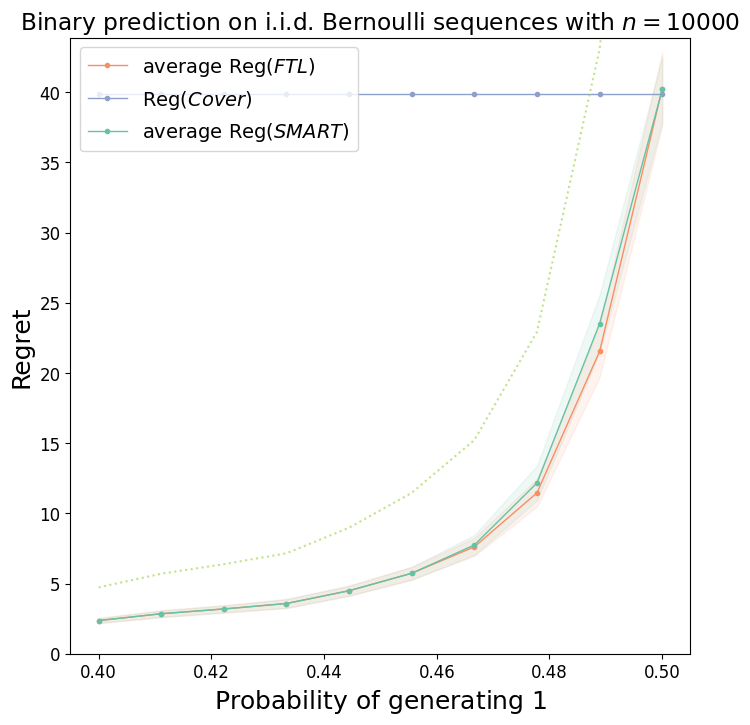
\includegraphics[width=\linewidth]{figures/detSMART_iid.png}
  \end{minipage}

  \vspace{0.6em}

  % Bottom: two side-by-side
  \begin{minipage}{0.48\linewidth}
    \centering
    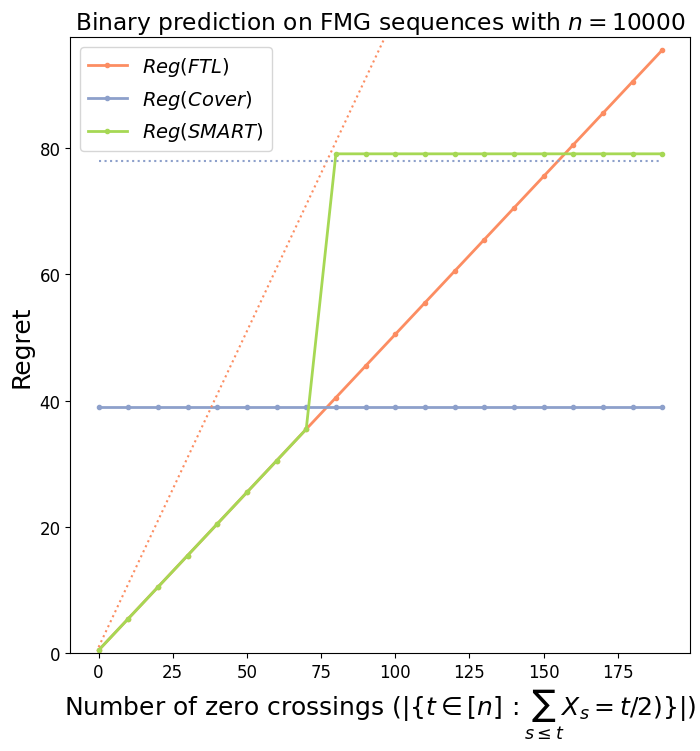
\includegraphics[width=\linewidth]{figures/detSMART_FMG.png}
  \end{minipage}\hfill
  \begin{minipage}{0.48\linewidth}
    \centering
    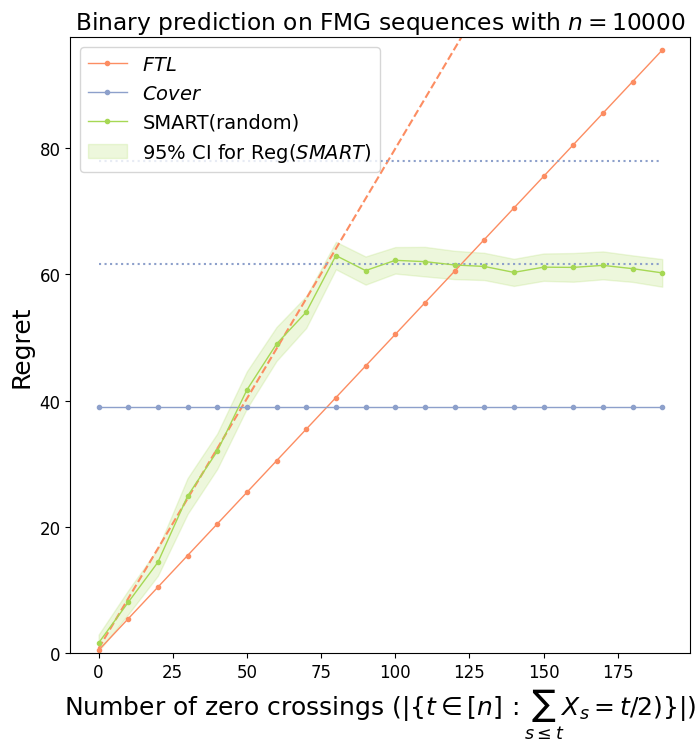
\includegraphics[width=\linewidth]{figures/randomSMART_FMG.png}
  \end{minipage}

  \captionsetup{format=plain}
  \caption{\it\footnotesize \raggedright Comparing the regret of $\ftl$, $\cover$ and $\bob$ on a collection of input sequences for fixed $n$.
  In Fig. $(a)$, we consider i.i.d. Bernoulli$(p)$ inputs for varying $p$. $\ftl$ and $\bob$ perform similarly, both achieving substantially lower regret than $\cover$ for $p<1/2$. 
  In Fig. $(b)$ and $(c)$, we consider `worst-case' binary sequences (as per~\cite{feder1992universal}) parameterized by the number of `lead-changes': the sequence with parameter $c$ comprises of $c$ pairs `$0,1$' or `$1,0$', followed by $n-2c$ `$1$'s. 
  In Fig. $(b)$, we consider $\bob$ with a deterministic switching threshold (\cref{thm:2ApproxRegret}) and compare $\Reg(\bob)$ with $2\Reg(\ftl)$ and $2\Reg(\cover)$ (dotted lines); in Fig. $(c)$, we use a randomized threshold (\cref{thm:SkiRentalRegret}), and show the average regret over the randomized threshold, as well as sample paths (plotted in green), and compare with $\frac{e}{e-1}$ times $\Reg(\ftl)$ and $\Reg(\cover)$ (dotted lines).}
  \label{fig:SMART}
\end{figure}



We also benchmarked performance against loss-based sequence generation as described by ~\cite{de2014follow}. Such sequences are constructed by initially alternating between the first and second expert and as time goes on, an extra copy of the first expert is appended every once in a while such that this expert slowly pulls ahead of the other. These sequences can characterized by this gap in loss between the two experts. A sequence designed to best approximate a particular gap as a function $f(n)$ is described to have ``loss-difference" function $f$. AdaHedge performs particularly poorly against a sequence with loss-difference $n^{0.4}$. The pseudocode to generate a sequence of length $n$ with a prescribed loss-difference is provided in~\cref{alg:LossDiffGeneration}; and to generate a $n^{0.4}$ sequence the loss-difference parameter is set to $n^{0.4}$. \cref{fig:SeqGeneration} illustrates how the difference in loss between two experts for a sequence generated this way roughly grows as the target of $n^{0.4}$. 

\begin{algorithm}[!h] 
\SetAlgoNoLine
\caption{Generating Loss-Based Sequences}
\label{alg:LossDiffGeneration}
\KwIn{Length $n$, \textsc{LossDiff}} 
\textbf{Initialize} $L_0 = L_1 = 0$, $t = 1$, seq = [ ]\;
\While{$t \leq n$}{
    \If{$|\textsc{LossDiff}(t) - (L_0 - L_1 - 1)| \leq |\textsc{LossDiff}(t) - (L_0 - L_1 + 1)|$}{
        Append 0 to seq\;
        $L_1 \mathrel{+}= 1$\;
    }
    \Else{
        Append 1 to seq\;
        $L_0 \mathrel{+}= 1$\;
    }
    $t = t + 1$\;
}
\end{algorithm}


\begin{figure}[!htbp]
  \centering
  \begin{minipage}{\textwidth} % Adjust the width as needed
    \centering
    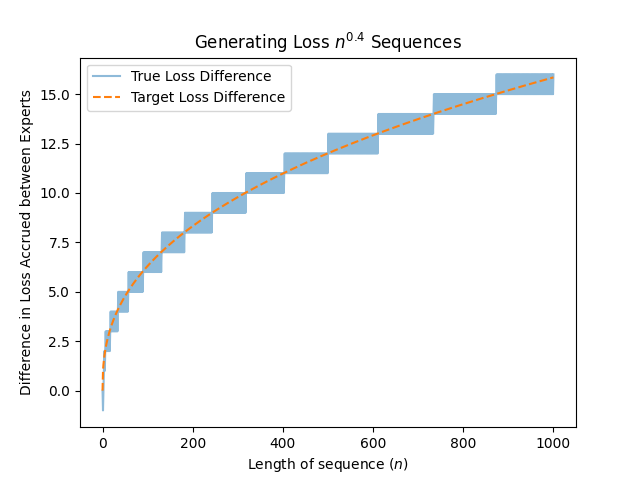
\includegraphics[width=0.8\linewidth]{figures/Loss-based_sequence_generation.png}
    %\caption{\it\scriptsize (a) $\bob$ with deterministic $\theta$, i.i.d. $y^n$}
  \end{minipage}%
  \hfill
\captionsetup{format=plain}
  \caption{\it\footnotesize \raggedright \it\footnotesize \raggedright Generating a $n^{0.4}$ loss-based sequence (as proposed in~\cite{de2014follow}). We show the characteristics of this sequence as constructed by iteratively appending $y_t \in \{0,1\}$ in an effort to best approach a loss-difference of $n^{0.4}$ (see~\cref{alg:LossDiffGeneration}).}
  \label{fig:SeqGeneration}
  \vspace{-0.5cm}  
\end{figure}


\cref{fig:SMARTBeatsAdaHedge} illustrates that on such $n^{0.4}$ loss sequences, AdaHedge (as well as $\cover$, which has regret growing as $\sqrt{\frac{n}{2\pi}}$ for all sequences) performs particularly poorly. On the other hand, $\bob$ (both with a deterministic and randomized threshold) achieves constant regret. 

\begin{figure}[!htbp]
  \centering
  \begin{minipage}{\textwidth} % Adjust the width as needed
    \centering
    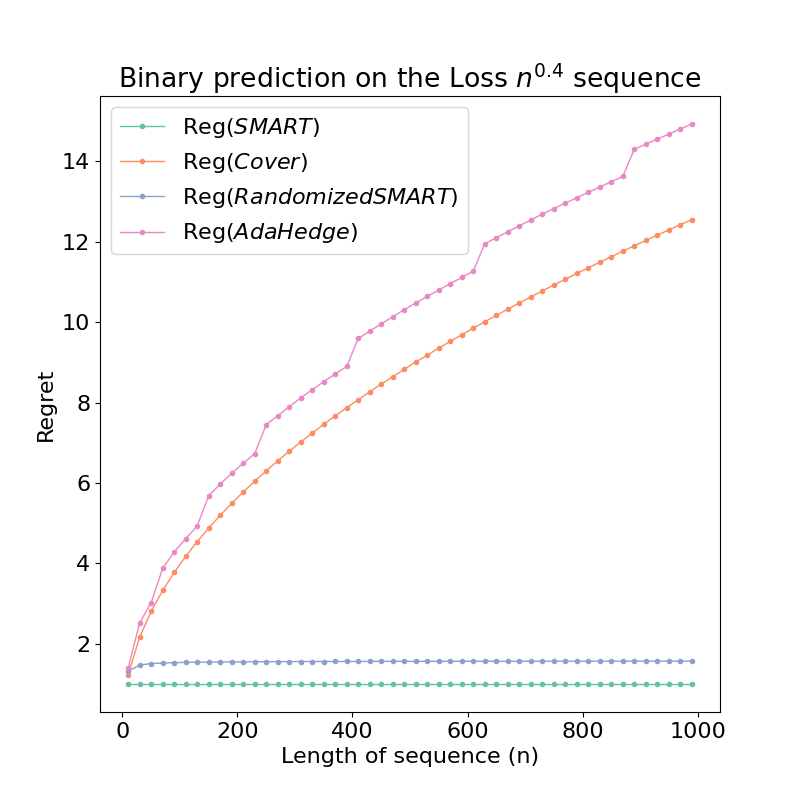
\includegraphics[width=0.65\linewidth]{figures/SMART_beats_AdaHedge.png}
    %\caption{\it\scriptsize (a) $\bob$ with deterministic $\theta$, i.i.d. $y^n$}
  \end{minipage}%
  \hfill
\captionsetup{format=plain}
  \caption{\it\footnotesize \raggedright Comparing regret of $\bob$, $\cover$, $\mathsf{Randomized}\bob$ and the $\mathsf{AdaHedge}$ algorithm on a  sequence with loss-difference $n^{0.4}$. We show the performance of each algorithm across different sequence lengths. The regret of $\bob$ and $\mathsf{Randomized}\bob$ are both constant order. $\mathsf{AdaHedge}$ performs worse than Cover, with both attaining $O(\sqrt{n})$ regret. }
  \label{fig:SMARTBeatsAdaHedge}
  \vspace{-0.5cm}  
\end{figure}

\color{blue}
Moving beyond binary prediction, we also evaluated SMART in the online linear classification setting. At each turn $t$, the learner is asked to provide a weight vector $x_t$ describing a separator between two labeled classes. In response, the learner receives a feature vector $z_t$ and a true label $y_t$, incurring loss $0.5 |z_t \cdot x_t - y_t|$. To keep the dot product bounded, $x_t$ and $z_t$ are restricted to be in the unit ball. 

In defining SMART for this setting, we use a regularized Follow the Leader algorithm (FTRL) provided in \cite{orabona2019modern} as the backup FTL. Orabona's algorithm is known to achieve less than $g(t) = \sqrt{2t}$ regret. In this experiment, we also explore empirically estimating $g(t)$ by measuring FTRL's regret against an adversarial sequence that repeatedly provides the same feature vector and randomizes the label. We find regret against the best constant-action weight vector by computing what FTL would have played had it known the next sample-label pair. 

We explored these three algorithms against four sequences: 1) Random i.i.d. 2) Massart noise 10\% 3) Label flips 4) Switching leaders. The "Random i.i.d." sequence is constructed by randomly generating a true $u$ separator, then selecting feature vectors from a standard normal, and finally providing correct labels relative to $u$. The "Massart noise 10\%" sequence is constructed similarly, with the additional detail that feature vectors have a 10\% chance of being mislabeled. In the "Label Flips" sequence, the feature vector remains the same at each step, while the label alternates on every turn. The "Switching leaders" sequence is constructed similarly, with labels alternating every 20 turns.   

\cref{fig:OLCComparison} illustrates the relevance of $\bob$ in applied settings. In generally representative sequences such as Random i.i.d. and Massart noise 10\%, $\bob$ exactly matches the strong performance of $\ftl$. In an adversarial case where the labels flip every turn and the leader is constantly changing, $\bob$ and $\bob$ with empirical-g are both able to avoid linear regret and play conservatively. $\bob$ with empirical-g experiences even less regret than $\bob$ by switching earlier than the $\sqrt{2t}$ threshold. In an adversarial case against FTRL with multiple leaders, $\ftl$ dominates, and both $\bob$ algorithms achieve great performance.     

\color{black}

\begin{figure}[!htbp]
  \centering
  \begin{minipage}{\textwidth} % Adjust the width as needed
    \centering
    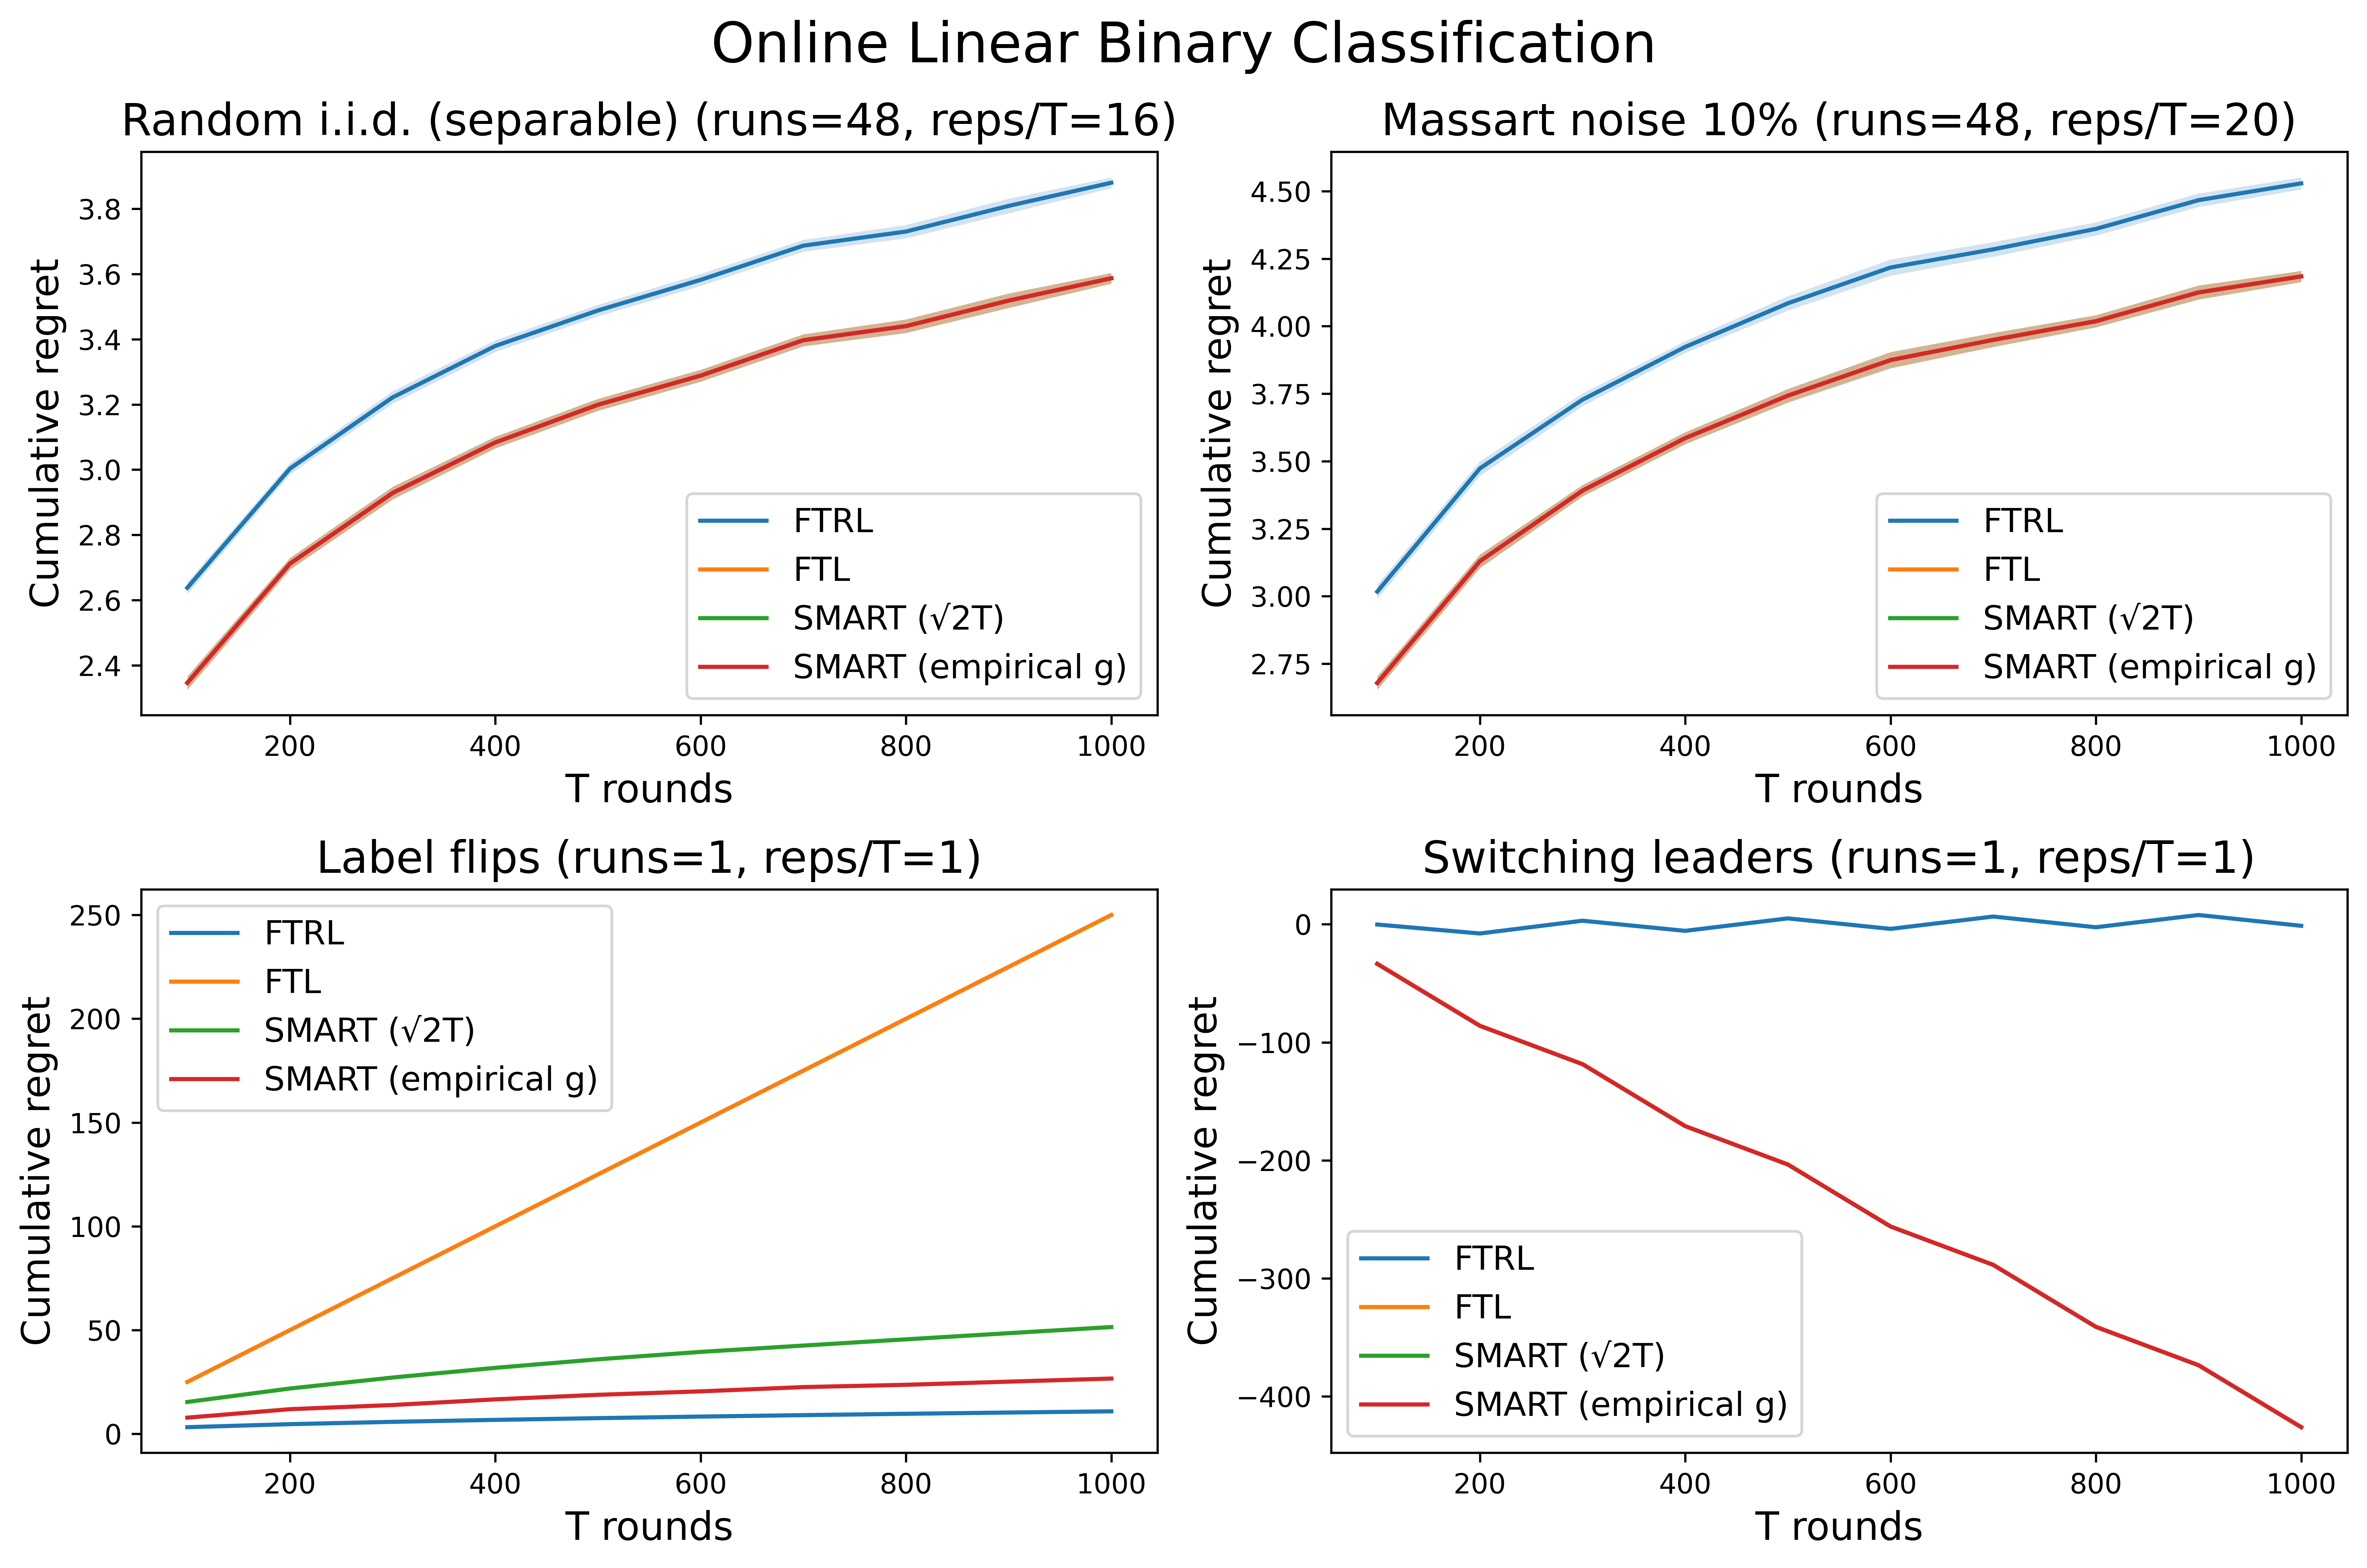
\includegraphics[width=0.95\linewidth]{figures/olc_comparison.png}
    %\caption{\it\scriptsize (a) $\bob$ with deterministic $\theta$, i.i.d. $y^n$}
  \end{minipage}%
  \hfill
\captionsetup{format=plain}
  \caption{\it\footnotesize \raggedright Comparing regret of $\ftl$, $FTRL$, $\bob$ and $\bob$ with empirical-g on 1) Random i.i.d, 2) Massart 10\% 3) Label flips 4) Switching leaders, across different sequence lengths. }
  \label{fig:OLCComparison}
  \vspace{0.5cm}  
\end{figure}